\documentclass[a4paper, 11pt]{article}

\title{Advanced Operating Systems 2011}

\author{Vivek Shah \\Department of Computer Science, ETH Zurich \\
\texttt{bonii@student.ethz.ch}}

%
% File: thesis_preamble.tex
%
% Author: Tim van Deurzen
% Date: 16/05/2010
%

\usepackage[svgnames]{xcolor}
%\usepackage[pdftex]{hyperref}
\usepackage{setspace}
\usepackage{url}
\usepackage{amsmath,amsfonts,amsthm,amssymb}
\usepackage{Tabbing}
\usepackage{fancyhdr}
\usepackage{lastpage}
\usepackage{extramarks}
\usepackage{chngpage}
\usepackage{graphicx,float,wrapfig}
\usepackage{fancybox}
\usepackage{listings}

\setlength{\parindent}{1.5em}

% Example environment.
\renewcommand{\labelenumii}{-}
\newenvironment{exmpl}{\begin{center}{\bf Example}\\\vspace{1em}\rule{0.75\textwidth}{0.8pt}\noindent}{\par\rule{0.75\textwidth}{0.8pt}\vspace{1em}\end{center}}

% Page margins.
\topmargin=-0.45in      %
\evensidemargin=0in     %
\oddsidemargin=0in      %
\textwidth=5.8in        %
\textheight=9.5in       %
\headsep=0.25in         %

% Set the spacing to leave 1.5 line open after each line.
\onehalfspacing

% Format any source code that is inserted.
\lstset{
    basicstyle=\footnotesize,
    keywordstyle=\color{NavyBlue}\bf,
    identifierstyle=\color{Black},
    commentstyle=\color{Green},
    stringstyle=\color{MidnightBlue}\ttfamily,
    showstringspaces=false,
    numbers=left,
    numberstyle=\footnotesize,
    numbersep=-1em,
    captionpos=b
}


\begin{document}
    
\maketitle
\newpage
\tableofcontents
\newpage

\section{Abstract}
As part of the course Advanced Operating Systems \cite{os-project},
the goal of the project is to build an operating system on top of the
minimal L4 microkernel \cite{l4}. The aim of the project is to build
the virtual memory system, file-system, system call interface, process
call interface, elf loader(to load executable files in ELF \cite{elf}
format from
the file-system) and a timer driver. It can be already seen that the
system can be perceived as quite modular where L4 provides the
necessary hardware abstraction and the other operating system features
are built up as multiple services over it which allows an ideal
composition of complexity(design of simple operation system) and
simplicity(services provided by L4). 

This report is divided into multiple sections. Firstly, I will give a
small introduction to the project which builds up on this
abstract. Then I will proceed to the technical details of the
interesting parts of the system to provide a broad insight into the
design and implementation of the system. I will point out any known
bugs/limitations in the system in the corresponding section. Finally,
I will try to sum up the overall picture of where the system stands
and hopefully it will not be obnoxious enough. 

\newpage
\section{Introduction}
Operating systems are considered to be the hobgoblins of systems. They
are almost inconspicuous and provide necessary abstractions to the application
programs. While monolithic kernel designs follow a very stringent
demarcation of a system and an application program, in a microkernel
approach this line becomes a bit blurred. In this project, a simple
operating system has been designed and implemented as a server on top
of the L4 microkernel whose services the client(application programs)
can access using the system call interface exposed in the file
``libs/sos/include/sos.h''.  In this project, the L4 Pistachio microkernel
\cite{l4-pistachio} has been used. The simple operating system({\bf SOS}) been
developed and tested using NSLU2 (Network Storage Link for USB 2.0)
disk drives \cite{slug} produced by Linksys. The device belongs to the
ARM architecture family \cite{arm-manual} and more details concerning
the hardware design are outlined in the hardware developer reference manual 
\cite{slug-manual}. There are some good references available for the
L4 microkernel which have been of great help in this project. The L4
user manual \cite{l4-usermanual} and the L4 kernel reference manual
\cite{l4-manual} are especially noteworthy.

SOS is a multi-threaded kernel(2 to be precise). One of the threads
has been designed to specifically handle system call messages(we will
refer to it as the rpc task). I will also use the term roottask for
the SOS kernel threads to avoid confusion since SOS is present atop L4 
microkernel. It is
the server to which the client programs using the sos library send
their service requests. All modes of data transfer between threads not
sharing address space use extensive message passing using L4 IPC
message passing mechanism. SOS implements the following operating
system features and/or abstractions over the L4 microkernel
\begin{itemize}
\item Virtual memory system, a virtual memory for the heap, stack and
  code segments with demand paging. Demand paging uses the second
  chance page replacement algorithm where the reference and dirty bits
  of pages are implemented in the software(pager). SOS uses an
  inverted page table design to achieve virtual memory support.
\item System call interface which is exposed to the application
  programs through the ``sos'' library which allows the
  applications(clients) to send specific service requests to the
  operating system.
\item File system interface which provides a file system abstraction
  over the low level NFS file system \cite{nfs-rfc} and converts the 
  asynchronous NFS
  operations into synchronous file operations as defined in the file
  system interface. It is important to note here that the SOS file
  system follows a flat directory structure.
\item A timer device driver which utilizes the timer hardware present
  in the NSLU2 slug in order to provide the time related system calls.
\item A process call interface which provides abstractions for the
  application programs to create, run, wait and kill processes which
  are binary images in the file system.
\end{itemize} 

\subsection{Segmentation of work by root-task threads}
As mentioned earlier, SOS is multi-threaded and it consists of 2 roottask
threads which are responsible for specific functionality. I will refer
them as the syscall loop thread and rpc thread. The rpc thread is
responsible for listening to system call requests from the client
processes. The syscall loop thread has the following responsibilities
\begin{enumerate}
\item Handling interrupts
\item Handling process kill message so that memory chunks of killed
  process are removed from page table. This message is sent by rpc
  thread. The rpc thread avoids doing this in order to avoid buffer locking
  problems.
\item Handling SOS library bootstrap message. When SOS library starts
  up it sends a message to its parent which is the syscall loop thread
  inquiring about the rpc thread id.
\item Handling message to flush all L4 mappings. This is not useful
  from the point of view of SOS anymore and is present as a vestige of a
  feature implemented as part of the pager milestone \cite{os-project2}.
\end{enumerate}
\newpage
\section{System calls}
System calls are mechanisms provided by the operating systems using
which client applications can request the operating system for
specific services. Since the client process is a different thread to
the operating system threads, it is a form of remote procedure call where the client
thread gets work done through the operating system threads. It
involves inter process communication between the client and SOS server
threads. There are situations where the system call invoked by the
client would need a series of asynchronous calls by the SOS server
threads for eg. NFS calls. In such situations, the roottask should not
block itself but rather the blocking would be done by the client
thread as it would wait for server thread to reply. The roottask only
replies when all the asynchronous work is done. The roottask would
service a specific system call completely if it needs no asynchronous
library calls even though there may be multiple concurrent system
calls. The system call interface is well defined in the form of the
services in the file ``libs/sos/include/sos.h''. The corresponding
client side implementation of the system calls is present in
``libs/sos/src/sos.c''. The corresponding server side implementation
and the headers are present in ``sos/sos\_rpc.c'' and ``sos/sos\_rpc.h''
respectively. The implementation and header of the callback functions used by the
server side system call are present in ``sos/sos\_rpc\_callbacks.c'' and
``sos/sos\_rpc\_callbacks.h''. 
\subsection{System calls Architecture}
The system calls proceed by message passing between the client sos
library and the rpc thread which is responsible for servicing those
system calls. Each message contains a label defined in
``helpers/ipc\_defs.h''. Based on the message label the rpc thread
identifies the type of the system call and takes the necessary
action. Since there is a limit on the amount of data that can be
packed in one message, some system calls send multiple messages to the
rpc thread to transmit the data and the server utilises a similar
mechanism where necessary. The client libraries present in
``libs/sos/src/sos.c'' first bootstraps itself to discover the rpc
thread id by sending a query message to the syscall loop thread. It
needs to do this since it needs to find the rpc thread id to which it
needs to send messages. For all system calls, the client library sends
a message to the rpc thread and blocks for a reply or multiple replies
until the system call is over. The rpc thread is responsible for
handling the system call messages directed towards it through the
\textit{rpc\_thread} function defined in ``sos/sos\_rpc.c''. This
function is responsible for determining the type of message and
delegating work to other helper functions. The basic architecture has
been outlined in figure \ref{systemcall-fig}.
\begin{figure}
\begin{center}
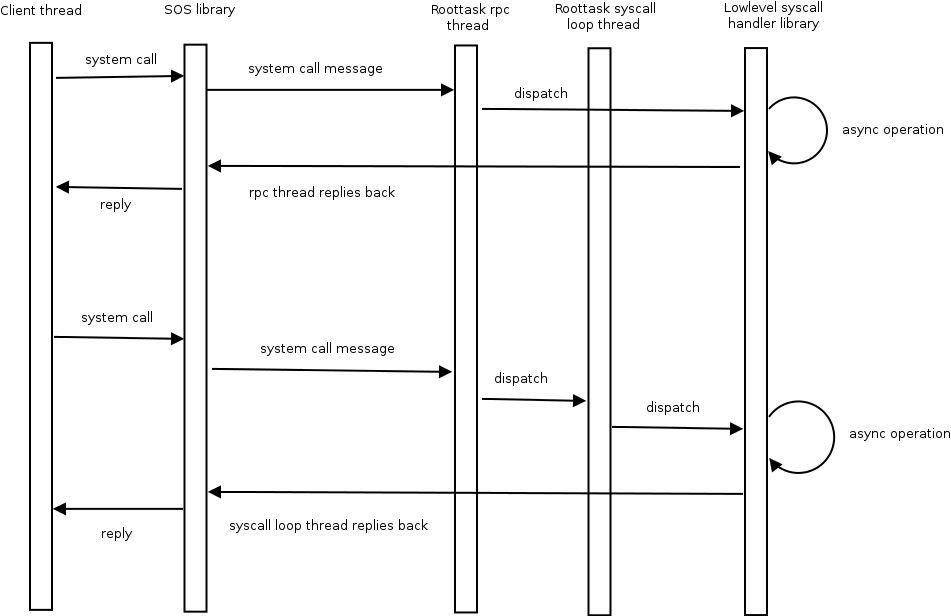
\includegraphics[scale=0.45]{systemcall.png}
\end{center}
\caption{System call handling architecture}
\label{systemcall-fig}
\end{figure}
In the figure \ref{systemcall-fig}, all messages from the client
library are shown as directed at the rpc thread. However, there is one
message which is sent to the syscall-loop thread which finds the rpc
thread id to which subsequent messages will be sent. This is
implemented in the ``sos\_init'' function which is defined in
``libs/sos/src/sos.c''. In some cases, the rpc thread replies back to
the client application while in other cases the syscall loop thread
replies back. A possible mechanism which can be exploited is to
forward the reply by the syscall loop thread to the rpc thread
however, there do not seem to be any immediately apparent advantage or
disadvantage of this approach and hence it has not been explored.

\subsection{Passing data in system calls}
In order to pass data in system calls, the data has to be passed
between two different L4 process, the client process and the rpc
thread. In order to do so, the inherent L4 message passing mechanism
is used. If a message can be packed into one L4 message then the message
is split and packed into multiple message registers of the L4 message
and sent else a message is split up into multiple L4 messages.
\subsection{File system interface}
SOS implements a flat file system atop the low level NFS file
system. It provides the necessary file system interface exported
through the system call interface. The file system interface is a
subset of the system call interface which allows the client library to
specify operations on the file. SOS implements the file descriptors
and the access permissions to them but it does not implement the low
level file structure in the file system. It uses NFS to do the low
level file manipulation for it. So, in a way SOS provides the file
descriptor view and access permissions and implements a blocking
interface for file operations as compared to the non blocking NFS
calls.

SOS handles regular files which are the files in the file system and a
console file which is the serial console for output and
input. Multiple processes can write to a console but only one process
can read from it currently. However, multiple process can read from
the console by changing the constants. A regular file can have
multiple processes reading and writing to it. It is to be noted though
that in SOS, when a file is opened for reading and writing, the
reading offsets and writing offsets are initialised at 0 and the end
of the file at the time of opening. Also, if a file is opened in read
mode, a size field at the time of opening the file determines the range
till where it must read. This size field is set to the size of the
file at the time of opening the file.

\subsubsection{File Descriptor Table}
SOS needs to store the file descriptors which the client library uses
to specify access to files. It also needs to maintain which threads
have access to which file descriptors so that there are no access
violations. For this it maintains a token table, file descriptors are
internally referred in SOS as tokens to reflect that processes must
hold specific tokens to access the resources. A token or file
descriptor is of type {\bf Token\_Descriptor\_t} and is defined in the
file ``sos/sos\_rpc.h'' and contains the following fields
\begin{enumerate}
\item The filename for which the token was issue.
\item Read and write count which contain the counts of the number of
  threads holding the token for read and write.
\item Access count which contains the total number of threads having
  access to the token. This is required as some threads can hold a
  resource both for reading and writing.
\item A list of access records which contains which thread has this
  token for read/write/both access and what are the specific write
  offsets and max read offsets for those threads. It is of type {\bf
    Token\_Access\_t} and is defined in the file ``sos/sos\_rpc.h''.
\end{enumerate}

\textit{Token\_Descriptor\_t contains a field token which is not used in
the code but was not removed from the existing code}. The token value
is an index so that a particular token can be identified in the token
table and also the thread which holds it, can be identified in the access
list of the token. So the actual token is a combination of 2 indices.

The file descriptor table is of static size and can be configured
through the constant ``MAX\_TOKENS''. In addition, there is a limit on
how many processes can access a token which can be configured through
the constant ``MAX\_ACCESSESS''. Both these constants are present in
the file ``sos/sos\_rpc.h''. The file descriptor table is manipulated
on receiving the open and close system calls.

\subsubsection{NFS library use}
Since SOS uses the NFS library for the low level file accesses, it is
careful to transfer small buffers for NFS read and writes. This is
necessary because otherwise NFS just ignores the request. Thus all NFS
read and writes are broken down to buffer size of 256 bytes. There was
no particular reason for choosing 256 other than it gave a
satisfactory performance and is an average buffer size i.e. neither
too big nor too small.

\subsubsection{Open and Close system calls}
When the client library issues an open system call, the rpc thread
checks if the resource has already been opened once. If not it tries
to allocate an entry in the token table. If the token table is not
full and the resource is not opened yet, it adds an entry for it and
adds the thread in its list of accesses, else the thread is just added
to the access list if the access limit is not violated. In case of
console access, the thread is registered in the list of listeners for
console interrupt if the open system call was issued for console
read. If the open system call was issued for a file which does not
exist in the file system then the file is created. The close system
call does the reverse where it removes the thread from the access list
of the token and also decrements the corresponding access, read and
write counts. In the token table, an entry is considered to be free if
the access count of the file descriptor is 0. 

 All the read and write
system calls first check if the thread requesting the resource with
the token actually have access to it. It also checks whether a thread
is trying to spoof a token it does not have. All the server end
implementation of system calls are present in the file
``sos/sos\_rpc.c''. I would not go into algorithmic description of the
other system calls as they can be easily followed from the code.

\subsubsection{Enhancement}
The server end implementation of ``sos/sos\_rpc.c'' utilises a lot of
repetitive messaging constructs which can be better structured but
need to be carefully thought out in the presence of global variables
and asynchronous calls. This should be done in SOS and can be viewed
as TODO which was not done owing to time constraints.

\newpage
\section{Clock Driver}
Device drivers are programs which allow higher level programs or
applications to interact with hardware devices. SOS implements a
simple clock driver to use the high resolution timer cells on the
slug. The timer registers in the slug are memory managed. The timer
registers are all present in the page {\bf NSLU2\_OSTS\_PHYS\_BASE}. The
details of the hardware are outlined in \cite[Page
  411]{slug-manual}. The memory managed registers used by SOS have
been defined below
\begin{itemize}
\item {\bf OSTS\_TS} is the timer register which gives the number of
  ticks elapsed.
\item {\bf OSTS\_STATUS\_REG} is the status register which is used to
  reset the status of the time stamp timer and the timer register. 
\item {\bf OSTS\_TIMER1\_RL\_REG} is the timer reload register which is
  used to set how after how long the interrupt will be generated to
  implement sleep queues. 
\item All the memory mapped registers mentioned above are offsets in
  NSLU2\_OSTS\_PHYS\_BASE page. However, the offset of OSTS\_TS is 0 and
  in \textit{time\_stamp} function instead of adding it to the page value, the
  page value is used directly. That does not affect the code
  functionality but affects readability. This has been noticed while
  writing the documentation and should be corrected.
\end{itemize}
The details of the clock driver and various pertinent implementation
specifics have been discussed in the following sections. The interface
for the client library is defined in the file
``libs/clock/include/clock.h''. The implementation of the defined
interface which is the device driver is present in
``libs/clock/src/clock.c''. It is to be noted that the device driver code
implemented in the previously mentioned file must be executed by a
privileged process and hence the roottask must execute it. The user
interface to the clock library are the {\bf time and sleep} system
calls which send a message to the rpc thread and then the rpc thread
executes the device driver library before replying back. 
\subsection{Registering Interrupts and Delegation}
A device driver functions through interrupt handling where one
specifies which interrupts are for a specific device. When L4 receives
interrupts for those device which have been registered with it, it
delegates the work to the interrupt handler. Since the syscall loop
thread is responsible for receiving registered interrupt messages from
L4 , it checks if the registered interrupts are for the timer
device. If it is so, it invokes the corresponding interrupt handler
routine in the clock driver based on the type of the interrupt. In
order to enable the clock driver interrupts, the clock driver
registers its interrupts with L4 at initialisation in the
\textit{start\_timer} function which is invoked by roottask while
bootstrapping. An interrupt by the timestamp timer indicates that the
timestamp timer has reached its maximum value and so the clock driver
must register the number of times the timestamp timer has completed
its cycle to compute the current time. An interrupt by the countdown
timer indicates it has counted down to 0. It is used to implement
sleep queues to set the time when the sleep queue must be examined to
wake up processes. These are the 2 interrupts that are registered by
the clock driver. The handler for timestamp timer interrupts is the
\textit{handle\_timer\_timestamp\_interrupt} function. It registers
the number of such interrupts received which will be used to compute
the timestamp value and resets the timestamp timer. The handler for
the timer interrupt is the \textit{handle\_timer\_interrupt} function
which determines if the sleep time of an entry in sleep queue is
over. In that case it sends the corresponding process a message to
wake up. Then, it determines, the time to count down for the next
timer interrupt to be generated and sets that value in the timer
register. It then resets the status reload register for the
countdown. Currently, in SOS the timer counts down with maximum
possible register value even if the sleep queue in empty. This should
be changed to disable the timer if the sleep queue is empty. This
would be more efficient.
\subsection{Sleep queue}
In order to implement the sleep system call, the clock driver needs to
maintain a list of processes which have issued the sleep system call
and their sleep times. It implements a sleep queue data structure
whose entry is of type {\bf sleep\_queue\_entry\_t} and is defined in
``libs/clock/include/clock.h''. It has the following fields
\begin{enumerate}
\item Tid of the sleeping process
\item Time when the process started sleeping (start\_time)
\item Time for which the process wanted to sleep (sleep\_time\_us)
\end{enumerate}
The queue is a FIFO queue where new sleep entries are registered at
the end of the queue. So, insertion in the queue is very quick. When a
timer interrupt is received, the entire list is searched for the
smallest sleep time remaining and the timer is set to that value. If
the value is greater than the timer's maximum countdown value then the
timer's maximum value is the countdown value. Also, if someone's sleep
time is over, that process is sent a wakeup reply message and evicted
from the sleep queue and the entire queue is compacted i.e. entries
after the evicted value are pushed up not to leave holes in
between. When a process invokes the sleep system call, the client
library sends a message to the rpc thread, the rpc thread checks if it
can add the entry to the sleep queue. If it can, it replies back to
the client application that it was registered and the client
blocks. The rpc thread in order to add the tid to sleep queue, checks
the min sleep time in the queue to include the possibility that the
new process being added can have a smaller sleep time than the
processes in the queue. If that is the case, it sets the timer
register accordingly for countdown. Also, since the syscall loop
thread receives interrupt messages, it is the syscall loop thread which
replies back to the sleeping thread for wake up. In hindsight,
compacting the queue is not a good idea, rather adding to the queue
can check the entire queue if an entry is available. That would be
much more efficient from a performance point of view. 
\subsubsection{Bugs}
Earlier, the syscall loop thread was responsible for adding entries in
the sleep queue and also evicting it, but now the rpc thread adds
entries in the queue while syscall loop evicts them. While
documenting, I noticed there is no locking done on the queue and this
might lead to race conditions. Also, the compaction is buggy in the
case where the entry which is next to the entry which is evicted is
ignored and not examined. This would lead to possible cases where the
entry next to evicted entry overshoots its requested sleep time.
This bug can be easily fixed by applying the simple
patch provided with this documentation
``0001-Fixed-entry-next-to-evicted-entry-not-examined.patch''. 
\newpage
\section{Memory System}
SOS has an available RAM of around 22 MB(on the slug) which it detects
while bootstrapping the roottask and divides it into frames
of size 4096 which is the page size. The page size is configurable. However,
it exposes a virtual memory of much larger size to the application
programs and provides this service using demand paging. There are
several page table designs which store the mapping from the virtual
memory address to the physical memory address mapping. For SOS, I have
chosen the inverted page table design. It is very scalable since it
scales according to the size of the physical memory instead of the
virtual memory. It is important to note that when a memory access
fault occurs (either the permission to access the memory location is
incorrect or the memory location is not present in L4 mappings), L4
kernel registers an interrupt and delegates this work to the root-task
syscall loop thread which is responsible for handling those interrupts
by invoking the pager method in ``sos/pager.c''. The memory pages have
been implemented as a linked list of frames where each frame contains
a link to the next available frame. This implementation of allocating
and de-allocating a frame is present in ``sos/frames.c''. The memory
systems also adds a guard page between the heap and stack which is
mapped to the physical address 0 and would fault when it is accessed.

\subsection{Page Table Structure}
SOS uses an inverted page table design which stores the virtual
address(page number) and process id. The index of the page table
stores implicitly the physical frame address. The inverted page table
design has been followed as outlined in the book
\cite[Page~395]{tanenbaum}.  Ideally it should be
hashed so that we must not do a lookup of the entire page table
however, owing to time constraints a hashed table has not been
implemented and a performance hit has been taken. On the positive
side, it can be argued that the design and implementation remains
simple and for a page table with around 5500-6000 entries which is the
case for the NSLU2 slug, the performance hit is not catastrophic.

The page table is not stored in the roottask's memory space but is
stored using the physical frames itself. It has been done because it
makes the system highly scalable even if there is a large amount of
memory available, the roottask's memory space remains free. Since the
size of the page table is not huge, storing it using the frames does
not cause available space issue. In addition the size of the page
table is computed dynamically using the the values of size of physical
memory available and the size of each page table entry. This generates
an optimum size of the page table which is then reserved using the
frames. 

Each page table entry is of type {\bf struct sos\_PTE} which in
addition to the virtual page number and the process id contains
additional helper structure for implementing demand paging. The
structure of the page table entry is documented in the header file
``sos/pager.h''. The swap table is an additional data
structure which contains entries pertaining to memory chunks which are
currently in the swap file and where are they present in the swap file.

\subsubsection{Advantages and Disadvantages}
An inverted page table design has all the advantages as mentioned in
the book \cite[Page~395]{tanenbaum}. What I would mention here are the
pros and cons of not having a hashed inverted page table. The
advantages are
\begin{enumerate}
\item The implementation is simple and fast.
\item For a small page table size the difference in searching the entire
  page table and some sections of the page table(hashed page table) is
  quite small if not negligible
\end{enumerate}
The disadvantages are
\begin{enumerate}
\item The system will not scale well in case of increased RAM.
\end{enumerate}
 
\subsection{Swap Table Structure}
Since the size of the physical memory is quite small compared to the
size of the virtual memory, sooner or later physical memory would be
completely used up while there would be demand for more virtual
memory. In such a case we would have to use a page replacement
algorithm where a page which is currently in the page table is evicted
from the page table and written to the swap and the new page which is
demanded is put in the page table. The swap table contains the mapping
of the virtual memory pages and the offset where they are currently in
the file. So, it can be viewed as a page table where we store the
offset in the filesystem instead of the physical address of the frame.

In principle, the page table datastructure can be used to store the
swap table entries as well but that is an overkill since the page
table datastructure contains additional helper structures for demand
paging which is not required for swap table. The swap table
datastructure is of type {\bf sos\_swap} which is documented in the
header file ``sos/pager.h''. Each swap entry, contains a link to the
index of the next free entry which gives performance speed up for
allocating and freeing a swap table entry. The size of the swap table
is also static and is configurable through the constant {\bf
  MAX\_SWAP\_ENTRIES} defined in ``sos/pager.h''. The swap file called
{\bf swapfile} is created in the NFS exported directory by the
roottask while bootstrapping. In case it is not created while
bootstrapping, the pager creates the file when it needs access to
it. The size of swapfile is upper bounded so each swap table entry
reuse their file offsets in the swapfile.

\subsubsection{Possible Design Issue and Enhancement}
When the swap table runs out of space i.e. all the swap table entries
are full then it cannot allocate the memory requested by the page
faulting process and hence the process would keep on page faulting
until some other process terminates it or some space in page table is
freed up. A possible enhancement can be to
decide whether to terminate the process or freeze it i.e. maintain a
list of such processes which are moved from run status to a non-run
status by not sending them a reply message. When an entry in swap or
page table frees up, they are moved from the non-run to run status.

\subsection{Demand Paging}
As we have seen previously, there would be scenarios where a page
table entry would need to be written to a swap file and read from it
when required. Based on the various order and type of memory accesses,
there can be multiple possible scenarios such as
\begin{enumerate}
\item Memory access where the access restrictions to the memory do not
  match
\item Memory access where the virtual memory is not mapped to the
  physical memory and there are available physical frames.
\item Memory access where the virtual memory is not mapped to physical
  memory and there are no available physical frames.
\item Memory access where the virtual memory is mapped to physical
  memory and the mapped page is present in page table.
\item Memory access where the virtual memory was mapped to physical
  memory and the mapped page is present in swap table and the page
  table is not full.
\item Memory access where the virtual memory was mapped to physical
  memory and the mapped page is present in swap table and the page
  table is full.
\end{enumerate}
The basic algorithm to handle the cases can be outlined by the
flowchart in figure \ref{pagefault-fig}. It is to be notes that the
roottask in the figure symbolizes the syscall-loop thread which is
responsible for handling interrupts for page faults. The algorithm also
handles cases where the low level swap file read and write can fail
owing NFS failure and handles those situations gracefully. For the
sake of clarity, those cases have not been depicted in the algorithm.
It is also to be noted, that although the NFS read and writes are
asynchronous the pager does not block until they are completed but
from the point of view of the application which page faulted it is
blocked since the roottask does not reply to it until it has resolved
the NFS reads/writes if issued. While the NFS read/writes are executed,
the corresponding page table entries are locked so that they are not
evicted by the page replacement algorithm as this will cause
inconsistent system state.
\begin{figure}
\begin{center}
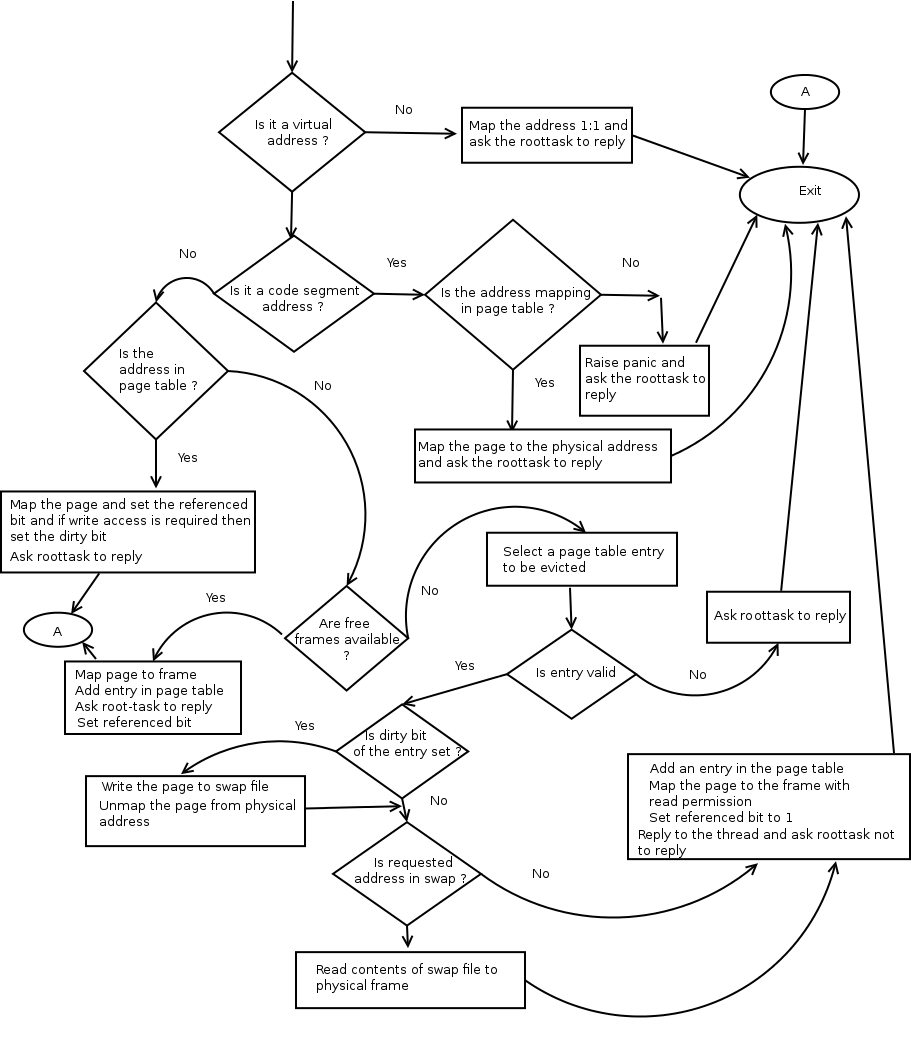
\includegraphics[scale=0.55]{pagefault.png}
\end{center}
\caption{Algorithm to handle page faults}
\label{pagefault-fig}
\end{figure}

\subsection{Implementing reference and dirty bits in software}
The algorithm outlined in figure \ref{pagefault-fig} details the broad
overview how page faults are dealt with demand paging. Since the ARM
hardware does not provide us with hardware managed reference and dirty
bits for pages, we need to do it ourselves. The dirty bit is set when
a page was written to since the time it was loaded from swap or loaded
for the first time. So, if a page is set without a write access, then
every write access to it would cause a page fault and hence we would
be able to set the dirty bit. This is precisely what is done in the
implementation. A page is provided with write access only if it is
present in the page table since then a page fault implies permission
fault. Whenever a page is mapped into the page table either for the
first time or from the swap, it is always mapped with only read
access. This keeps the algorithm logic simple. The only down-sight to
it is that if the first access to a page is write access, it will be
mapped through 2 page faults but that is not a big performance
delimiter. A page is considered to be referenced whenever any access
is made to it. This reference bit is used by the second chance page
replacement algorithm to determine the page table entry that would be
evicted.

\subsection{Page Replacement Algorithm}
For the algorithm presented in figure \ref{pagefault-fig}, it is
important to select a suitable target page table entry which needs to
be evicted. SOS implements a second chance page replacement algorithm
as described in \cite[Page~399]{tanenbaum}. This algorithm checks the
reference bits and if a page was referenced then it is given a second
chance and not evicted but the reference bit is cleared. A page with a
clear referenced bit is evicted. In addition, a pinned bit is present
for each page table entry to signify that the corresponding entry
should never be evicted. It is not the same as page table entry lock done
on read and write to swap file. The implemented algorithm can be
outlined by the following steps
\begin{enumerate}
\item Iterate over the page table entries infinitely. For each entry
\item Check if the reference bit is 0. If the reference bit is 0 and
  the page pinned bit is 0 and the page table entry is not being
  currently updated then return the page table entry as the entry to
  be evicted else go to next step.
\item If the page table entry is not being updated and the reference
  bit is set to 1 then clear the reference bit and unmap the page so
  that we can know if it is referenced through a page fault.
\item If all the page table entries in a full cycle of traversal are
  being updated then exit from loop with an invalid index to signal no
  entry found for eviction else the algorithm will be stuck in
  infinite loop as it will not be able to service the NFS callbacks
  which are the only way a page table update lock can be freed up.
\end{enumerate}
The page replacement algorithm is quite simple to understand and easy
to implement. Every invocation of the algorithm begins the search from
the index where it terminated in the previous invocation and this can
be easily achieved using a static variable.

\subsubsection{Bug}
If all the pages in the page table are pinned then the algorithm would
go into infinite loop. This bug has been discovered right now while
looking at the code for documentation. It can be easily fixed by
adding a simple condition to check that if all page table entries in a
full cycle of traversal are being updated or pinned then the algorithm
must abort. The current implementation just checks whether all the
entries are being updated and not for pinned. 

\subsection{Write to swap and Read from swap}
The NFS read and writes are asynchronous and they need to be done
in small chunks rather than a huge chunk all at once. In SOS, NFS read
and writes are done in chunks of 256 bytes. While the roottask pager
method cannot block for completion of NFS read/writes, the page
faulting application must block until the corresponding read and
writes are completed. This is solved by using callback functions. On
NFS read write completion the associated callback function is
executed. In order to maintain state so that corresponding action can
be taken on receiving callbacks, the necessary state information is
passed as tokens to the NFS read and write calls. On completion of the
NFS read and write calls, the corresponding callbacks are invoked with
the appropriate tokens. The token used for a swap write and swap read
is of type {\bf struct page\_token}. Its fields have been documented
in the file ``sos/pager.h''. In case of a swap write followed by a
swap read, the swap write callback issues the necessary NFS
read. While the swap write and/or read are performed, the page table
entries are locked so that they are not evicted(used) for other page
faults. 
\subsection{Pinning pages}
Page table entries can be marked as pinned so that they cannot be
evicted. If a page is marked as pinned then the page replacement
algorithm ignores them and does not consider them for eviction. Such
pinning is useful for preventing eviction of memory buffers in
asynchronous requests so that those buffers are not paged
out. Also, code segment pages are pinned in the page table. Currently,
in SOS no method has been exposed to allow client libraries to pin
memory buffers in asynchronous requests owing to time constraints but
they can be easily added since the pinning mechanism is already in place.
\newpage
\section{Process Management}
In SOS every process is a single thread of execution. A process does
not have more than one thread of execution. In SOS, each process is a
L4 thread. The process abstraction presents an abstracted view to the
client application and presents a convenient interface to
manipulate process states. PID or the process identifier is the
abstraction provided to the client to reference a specific process in
SOS. The various process states are
\begin{enumerate}
\item Created - The process has been created but it cannot run since
  its code segment has not been loaded.
\item Ready - The process is ready to run.
\item Waiting - The process is waiting for some other or any process
  to terminate.
\item Sleeping - The process wants to wait for a specific time
  interval rather than on process termination.
\item Killed - The process has been removed from the system. Its code
  segment has been unloaded and the memory it occupied has been
  removed.
\end{enumerate}

\begin{figure}
\begin{center}
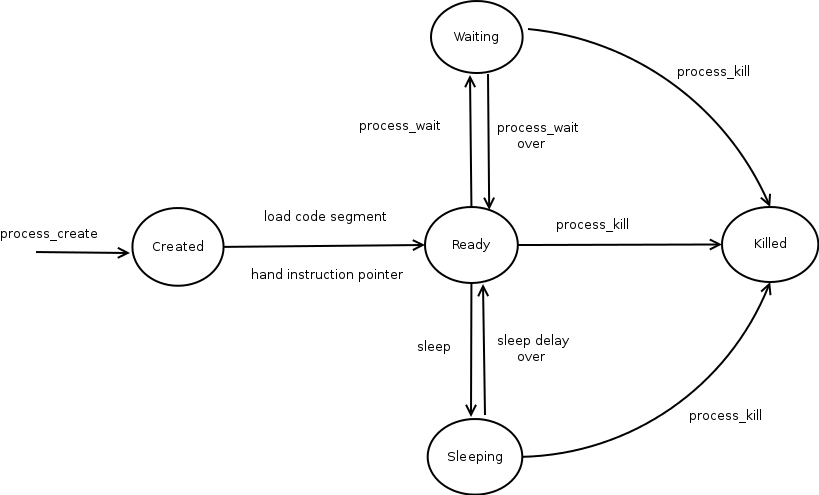
\includegraphics[scale=0.5]{process-states.png}
\end{center}
\caption{Process states}
\label{process-states-fig}
\end{figure}

The possible transitions among these process states in SOS can be
depicted by figure \ref{process-states-fig}. The edge labellings
depict the library bindings available for the process state
manipulation. It is important to remember here that a process can wait
for another process which is specified through the PID or a PID value
of -1 indicates that a process wants to wait for any process to
terminate. It is also important to remember that a process\_delete can be
issued by a process to kill any other process but a process\_wait and
sleep are only invoked on the calling process to change its status
from ``Ready'' to ``Waiting'' and ``Sleeping'' respectively. 

\subsection{Process Memory View}
As outlined previously, SOS supports a virtual memory layout where the
user heap and stack present a large virtual memory than the actual
main memory present. In addition, the executables are loaded from the
file system into the code segment of the memory layout. The view of
the memory layout to the process is depicted in figure
\ref{process-memory-fig}.
\begin{figure}
\begin{center}
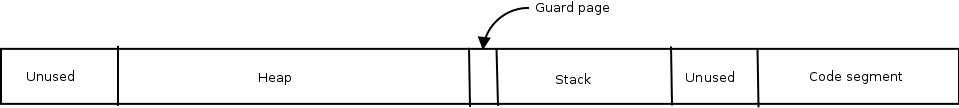
\includegraphics[scale=0.4]{memory-layout.png}
\end{center}
\caption{Process memory view}
\label{process-memory-fig}
\end{figure}
The memory layout has the following characteristics
\begin{enumerate}
\item The heap segment starts at the virtual address 0x2000000 and
  extends up to 0x7000000. The stack grows down from 0x7750000. The
  guard page is present at 0x7000000 to guard against stack overflows.
  The heap configuration can be easily adjusted by modifying the
  register values in ``libs/c/crt/sys-sos/arch-arm/crt0.S''. The stack
  value can be modified by changing the constant {\bf stack\_address}
  in ``sos/sos\_rpc\_callbacks.c''.
\item The code segment starts from 0x10000000. This is done by specifying
  the -Ttext param in the top level SConstruct and the pager
  interprets all virtual addresses above this as the code segment. The
  elf loader is responsible for loading the binary elf file from the
  file system and expanding it in memory. This happens during the
  process\_create call and is explained in details later.
\item The virtual memory design is currently only experimental as is
  evident from the small size and from unused regions. The size can be
  easily adapted by modifying the constants for later enhancements.
\end{enumerate}
\subsection{Process Table Structure}
The process management needs to maintain a process table where each
entry of the table is a helper datastructure containing the relevant
information of the process. This is the process control block and is
of type {\bf process\_control\_block\_t}. It contains
\begin{enumerate}
\item Thread id of the process in the system.
\item List of process ids waiting for it to terminate.
\item Tokens which the process holds.
\item Helper fields useful for process detail output. 
\end{enumerate}
The process control block and its fields are documented in the file
``sos/sos\_rpc.h''. The process table is a static array whose size can
be controlled by the value of constant {\bf MAX\_PROCESSES} defined in
the same header file as mentioned above. The PID of a process is the
index of the process control block in the process table. The process
control block in SOS does not contain any process hierarchies.
\subsection{Process Creation and Elf Loading}
On process creation, the requested binary image needs to be read from
the file system using a series of asynchronous NFS\_reads and when the
entire data(elf file) is loaded into memory it needs to be loaded into
the code segment and then run. It is important to note that the
process is first created i.e. its entry in the process table is filled
out and then it loaded from the file system before being run. In case
the load from the file system and/or running the process fails,
its entry is removed from the process. The entire sequence of steps
has been depicted in figure \ref{elf-loading-fig}.
\begin{figure}
\begin{center}
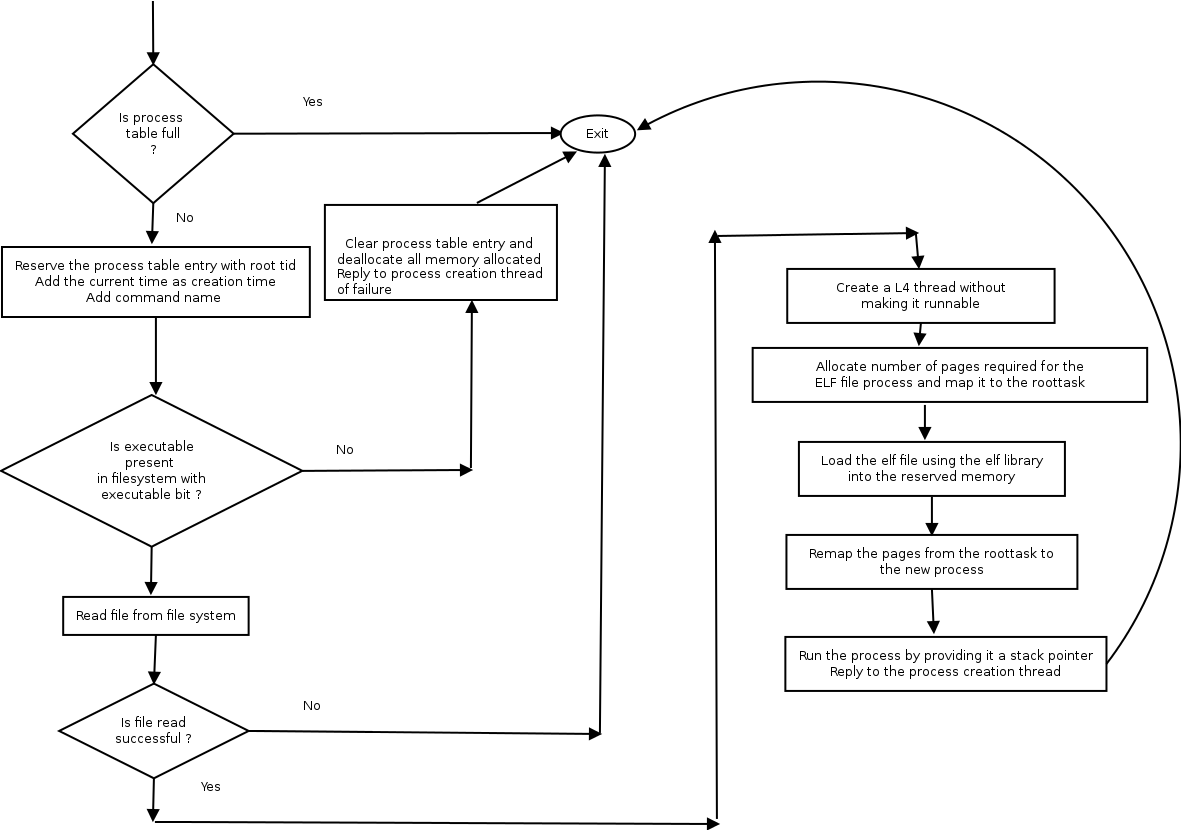
\includegraphics[scale=0.4]{process-creation.png}
\end{center}
\caption{Process creation using ELF loading}
\label{elf-loading-fig}
\end{figure}
There are some interesting details about process creation which are
\begin{itemize}
\item The ELF loader only loads file which have executable bits in the
  file system. Copying files by the project builder somehow strips the
  files of the executable bits and hence their executable bits must be
  set prior to run.
\item The ELF loader loads the entire executable file into the code
  segment at once.
\item The code segment entries are pinned in the page table and hence
  they cannot be evicted.
\item The ELF loader first reserves memory chunk to read in the file
  from the filesystem. Then it reserves pages in the pagetable to
  expand the read ELF file using the native ELF library. Since the
  entire relocated ELF during the build process is generated with
  addresses in the code segment of virtual memory, reserving memory in
  the code segment is quite easy.
\item Before invoking the ELF library, the code segment memory pages
  are mapped to roottask so that the ELF library can easily access
  them. Once the expansion of ELF image is complete, the code segment
  pages are mapped to the newly created process.
\end{itemize}
The above mentioned elf loading into main memory is done by
``load\_code\_segment\_virtual'' function in ``sos/pager.c''.
\subsubsection{Advantages and Disadvantages}
The advantages of this approach are
\begin{enumerate}
\item It is simple to understand and implement. 
\item It does not cause any complicated what if conditions which need
  to be thought out.
\end{enumerate}
The disadvantages of this approach are
\begin{enumerate}
\item It is quite wasteful of memory as the code segment can be loaded
  and unloaded on demand.
\item Pinning the pages causes a lot of page table entries to be
  blocked out when an alternative approach can make it work in a much
  more efficient manner.
\end{enumerate}
The decision for SOS to support a simple ELF loading as outlined above
was taken because it was quite efficient to implement within the time
constraints available and worked well for the specification.
\subsection{Process Wait}
A process can switch from the ``Ready'' state to ``Waiting'' state by
issuing a process\_wait call. It can wait for a particular process to
terminate or for any process in the system to terminate. On issuing
process\_wait the issuing process waits for a reply back from the rpc
thread. The rpc thread on getting a process\_wait call adds the
process to the list of waiting processes in the process control block of the
process for which the callee wants to wait. If the callee wants to
wait for a process with PID -1, it is appended to the
any\_process\_list and any process when it terminates it sends a reply
back to the processes in its waiting process list and to the processes in the
any\_process\_list. Thus process wait is a mechanism in SOS using
which different processes can establish dependencies among themselves
and wait for execution of other such processes to complete.
\subsection{Process Delete}
This is the mechanism by which a process switches from any state to
the ``Killed'' state. Since there is no process hierarchy in SOS, a
process can invoke a process\_delete on any other process. When a
process terminates normally without a kill issued on it in SOS, it
issues a process\_delete on itself. On receiving a process\_delete,
SOS does the following
\begin{enumerate}
\item Kill the L4 thread.
\item Close all the page tokens held by the process.
\item Release all memory held by the process i.e. from the page table
  and the swap table.
\item Free the process control block.
\item Remove the process from the list of waiting processes for any
  process in the process table.
\item Send a reply message back if the process delete was not issued
  by a process on itself.
\end{enumerate}
\subsection{Additional housekeeping by process control block}
Since the process control block maintains information pertaining to
the list of open tokens for file access, the process control block of
a process is updated on every file open and close system call to
maintain a consistent current open tokens information structure. In addition,
every process also maintains the size in pages of the virtual memory
occupied by it(heap and stack). So every allocation and deallocation
by the pager where it allocates or deallocates a page table entry
correspondingly updates the size in the process control block. This
provides a dynamic view of main memory occupied by a process. 
\newpage
\section{Acknowledgment}
Developing SOS has not been a trivial task and it has had its fair
share of sleepless nights, frustrated keyboard banging and Eureka
moments. I would like to acknowledge the help and effort put in by
Frederik Mutzel with whom I was initially working on the project. He
had to drop out owing to health concerns but a lot of the initial
design was done in conjunction with him. I would also like to
acknowledge the help of Praveen Shinde and Simon Peter who have always
helped in providing the right direction and been flexible enough when required.
\newpage
\bibliographystyle{abbrv}
\bibliography{report}
\end{document}
